%% REPLACE SXXXXXX with your student number
\def\studentNumber{S2816575}


%% START of YOUR ANSWERS
%% Add answers to the questions below, by replacing the text inside the brackets {} for \youranswer{ "Text to be replaced with your answer." }. 
%
% Do not delete the commands for adding figures and tables. Instead fill in the missing values with your experiment results, and replace the images with your own respective figures.
%
% You can generally delete the placeholder text, such as for example the text "Question Figure 2 - Replace the images ..." 
%
% There are 18 TEXT QUESTIONS (a few of the short first ones have their answers added to both the Introduction and the Abstract). Replace the text inside the brackets of the command \youranswer with your answer to the question.
%
% There are also 3 "questions" to replace some placeholder FIGURES with your own, and 3 "questions" asking you to fill in the missing entries in the TABLES provided. 
%
% NOTE! that questions are ordered by the order of appearance of their answers in the text, and not by the order you should tackle them. Specifically, you cannot answer Questions 2, 3, and 4 before concluding all of the relevant experiments and analysis. Similarly, you should fill in the TABLES and FIGURES before discussing the results presented there. 
%
% NOTE! If for some reason you do not manage to produce results for some FIGURES and TABLES, then you can get partial marks by discussing your expectations of the results in the relevant TEXT QUESTIONS (for example Question 8 makes use of Table 1 and Figure 2).
%
% Please refer to the coursework specification for more details.


%% - - - - - - - - - - - - TEXT QUESTIONS - - - - - - - - - - - - 

%%Question 1 - Explain what these figures contain and how the curves evolve, and spot where overfitting occurs. Reason based on the min/max points and velocities (direction and magnitude of change) of the accuracy and error curves

%% Question 1:
\newcommand{\questionOne} {\youranswer{the \emph{training accuracy} increases steadily throughout training, eventually approaching a high value close to saturation ($\sim0.950$). In contrast, the \emph{validation accuracy} initially increases but then plateaus and starts decreasing around epoch $\sim5-10$, after which it fluctuates slightly without any further systematic improvement. At the final epoch, the validation accuracy is around $\sim0.810$, which is a significant decrease. Figure~\ref{fig:example_errorcurves} presents the corresponding cross-entropy errors. The \emph{training error} decreases monotonically, while the \emph{validation error} initially falls but then stops decreasing and begins to level off around the same epoch range ($5-10$). From that point onward, the training error continues to decrease whereas the validation error begins to steadily increase. This divergence between the training and validation curves indicates an increasing \emph{generalisation gap}, which is the difference between the validation error and training error. The generalization gap at the final epoch is around $\sim1.5$. The model fits the training data more and more closely but no longer improves. This is a clear indication of overfitting, as the model is learning the training data too well and is not generalising to the validation data.}
}



%Question 2 - Present your network width experiment results by using the relevant figure and table

%% Question 2:
\newcommand{\questionTwo} {
\youranswer{varying the number of hidden units has a clear impact on both performance and overfitting. Table~\ref{tab:width_exp} and Figure~\ref{fig:width_acccurves} show that the network with $32$ hidden units achieves the lowest validation accuracy ($72\%$) and the highest validation error ($0.700$), while the models with $64$ and $128$ hidden units perform better on the validation set. In particular, the $128$-unit model attains the smallest training error at the end of training, $0.156$. However, Figure~\ref{fig:width_errorcurves} also reveals that the $128$-unit model exhibits a larger gap between training and validation error: its training error continues to decrease while the validation error flattens and rapidly increases after around epoch $\sim 5$. This indicates stronger overfitting compared to the $64$-unit model, whose training and validation errors remain closer together, though the validation error does increase after epoch $\sim 60$, albeit at a slower rate, indicating overfitting in that case as well. The $32$-unit model shows little signs of overfitting, having a generalization gap of around $\sim 0.1$ at the final epoch. Thus, while increasing width from $32$ to $128$ hidden units improves validation accuracy, it also amplifies the generalisation gap, with the widest model overfitting the most.}
}

%Question 3 - Discuss whether varying width affects the results in a consistent way, and whether the results are expected and match well with the prior knowledge (by which we mean your expectations as are formed from the relevant Theory and literature

% \youranswer{Our findings clearly indicate that varying the number of hidden units affects the results in a consistent manner. As we increase the number of hidden units from 32 to 64, we observe an improvement in validation accuracy from 78.4\% to 80.7\%, and a corresponding decrease in both training and validation error. This trend continues as we further increase the hidden units to 128, where we achieve a validation accuracy of 80.2\%. However, it is important to note that while the training error decreases significantly with more hidden units, the validation error does not follow the same trend, indicating potential overfitting at higher capacities. These results align well with established theories in neural network literature, which suggest that increasing model capacity can lead to better performance up to a certain point, beyond which overfitting may occur if not properly regularized. Overall, our expectations based on prior knowledge are confirmed by our experimental results}
%% Question 3:
\newcommand{\questionThree} {
\youranswer{Our width experiment confirms the expected trade-off between model capacity, performance, and overfitting. As we increase the number of hidden units from $32$ to $64$ and $128$, training error decreases monotonically and training accuracy increases (or stays around the same in the case of the $128$- and $64$- unit models), showing that wider networks fit the training data more easily. Validation performance initially benefits from this increase in capacity: moving from $32$ to $64$ hidden units improves validation accuracy and reduces validation error. However, beyond a certain point, additional capacity primarily reduces training error without translating into better validation performance. In our results, the $128$-unit model achieves the lowest training error but exhibits a larger generalisation gap of around $\sim0.8$. This is significantly larger than the $64$-unit model(gap around $\sim0.4$). Consequently, the $128$-unit model overfits more than the $64$-unit model, even though it has the best training performance. The $64$-unit model provides a better balance between training fit and generalisation, overfitting less while still outperforming the $32$-unit model on the validation set. This behaviour aligns with standard bias-variance and capacity arguments in the neural network literature. Increasing capacity reduces bias~\footnote{Here, bias can be defined as $
    \text{bias}(\hat{\theta}_m) = \mathbb{E}[\hat{\theta}_m] - \theta_m  
$ where $\hat{\theta}_m$ is the expecation over the dataset and $\theta_m$ is the true underlying function to be learned.} but increases variance \footnote{
    $Var[\hat{\theta}]$, where $\hat{\theta}$ is the estimator. The variance of an estimator provides a measure of how we would expect the estimate we compute from data to vary as we independently resample the dataset from the underlying data-generating process.
} and the risk of overfitting if regularisation is insufficient (e.g. \cite{Goodfellow-et-al-2016}, chapter $5.4.4$). Our empirical findings match these theoretical expectations moderate width improves generalisation, whereas excessive width mainly amplifies overfitting.}
}

% Question 4 - Present your network depth experiment results by using the relevant figure and table
%% Question 4:\youranswer{varying the number of hidden layers has a significant ($\sim0.3$ difference in final validation error values) on the error and accuracy curves. We observe that the final training error value for the $3$ hidden layer model is the lowest at $0.160$, while the final validation error is the highest at $1.209$. This indicates that the model has overfit to the training data. In contrast, the $2$ hidden layer model achieves the highest validation accuracy of $81.0\%$ and a lower validation error of $0.927$. The $1$ hidden layer model performs the worst overall, with a validation accuracy of only $68.3\%$ and a high validation error of $1.163$. These results suggest that increasing depth can improve performance up to a point, but excessive depth may lead to overfitting if not properly managed}
\newcommand{\questionFour} {
\youranswer{varying the number of hidden layers also affects both performance and overfitting. Table~\ref{tab:depth} and Figure~\ref{fig:depth_acccurves} show that a network with only $1$ hidden layer underperforms: it attains the lowest validation accuracy and the highest validation error, and both training and validation errors remain relatively high, indicating underfitting.

Adding more depth improves validation performance. The $2$- and $3$-layer networks achieve substantially higher validation accuracy and lower validation error than the $1$-layer model. However, Figure~\ref{fig:depth_errcurves} reveals that the deeper networks also display larger gaps between training and validation error. For the $3$-layer model in particular, training error continues to decrease while validation error plateaus or slightly increases after around epoch~[X], indicating stronger overfitting. The $2$-layer model offers a better compromise, showing improved validation performance over the $1$-layer baseline while maintaining a somewhat smaller generalisation gap than the $3$-layer model. Overall, depth improves representational power but also increases the tendency to overfit.}
}

% Question 5 - Discuss whether varying depth affects the results in a consistent way, and whether the results are expected and match well with the prior knowledge (by which we mean your expectations as are formed from the relevant Theory and literature
%% Question 5:
\newcommand{\questionFive} {
\youranswer{Our findings indicate that varying the number of hidden layers affects the results in a consistent manner. As we increase the depth from 1 to 2 hidden layers, we observe a significant improvement in validation accuracy from 68.3\% to 81.0\%, along with a corresponding decrease in both training and validation error. This trend suggests that adding more layers allows the model to capture more complex patterns in the data, leading to better generalization. However, when we further increase the depth to 3 hidden layers, we notice a slight increase in validation accuracy to 81.7\%, but also a substantial increase in validation error to 1.209, indicating overfitting. These results align with established theories in neural network literature, which suggest that while increasing depth can enhance model capacity and performance, it also raises the risk of overfitting if not properly regularized. Overall, our expectations based on prior knowledge are confirmed by our experimental results}
}


%% Question 6: Explain how one could use a combination of L1 and L2 regularisation. Discuss any potential benefits of this approach. Present an equation for this combined loss function and explain all relevant variables and hyperparameters.

% \youranswer{
    % We consider a combined regularisation approach that incoporates both L1 and L2 penalties to leverage the strengths of each method. A naive combination would simply add both penalties to the loss function, namely: 
    % \begin{equation}\label{eq:L1L2Naive}
    %     \mathcal{L} = \mathcal{L}_{CE} + + \lambda ||w||_1| + \lambda ||w||^2_2
    % \end{equation}
    % where $\mathcal{L}_{CE}$ is the cross-entropy loss, $w_i$ are the model weights, and $\lambda$ is a hyperparameter controlling the strength of the penalization. While this approach is straightforward, it may not fully exploit the complementary benefits of L1 and L2 regularisation. The gradient contributions from both penalties could interfere with each other, potentially leading to suboptimal weight updates.

    % % Get the adam rule and add each component,
    % Using Adam's Learning rule, the gradient update for weight $w_i$ at time step $t$ would be: 
    % \begin{align*}
    %     m_t & = \beta_1 m_{t-1} + (1 - \beta_1) \nabla_{w_i} \mathcal{L} \\
    %     v_t & = \beta_2 v_{t-1} + (1 - \beta_2) (\nabla_{w_i} \mathcal{L})^2 \\
    %     \hat{m}_t & = \frac{m_t}{1 - \beta_1^t} \\
    %     \hat{v}_t & = \frac{v_t}{1 - \beta_2^t} \\
    %     w_i & = w_i - \eta \frac{\hat{m}_t}{\sqrt{\hat{v}_t} + \epsilon}
    % \end{align*}
    % where $\eta$ is the learning rate, $\beta_1$ and $\beta_2$ are the exponential decay rates for the moment estimates, and $\epsilon$ is a small constant to prevent division by zero. We have: \begin{align*}
    %     \nabla_{w_i} \mathcal{L} & = \nabla_{w_i} \mathcal{L}_{CE} + \lambda \cdot sign(w_i) + 2\lambda w_i
    % \end{align*}
    % % Show that L1 and L2 to not contribute equally
    % Thus, we see that the L2 regularisation term scales with the weight magnitude, while the L1 term contributes a constant gradient based on the sign of the weight. This means that for small weights, the L1 term will dominate, promoting sparsity, while for larger weights, the L2 term will have a more significant effect, encouraging smaller weight magnitudes. However, since we start with small weights and L2 continuously tries to keep them minimized, L2 may struggle to have a significant effect unless weights grow larger during training, potentially limiting the benefits of L2 regularisation.
    % % Propose adding another hyperparameter which is the balance /reference the original paper
    % To mitiage these issues, we apply Elastic Net reguralisation, which combine the L1 and L2 penalties in a weighted manner~\cite{L1L2_combined}:
    % \begin{align}
    %     \mathcal{L} = \mathcal{L}_{CE} + + \lambda (\alpha ||w||_1|) + \lambda ((1 - \alpha ) \frac{1}{2} ||w||^2_2)
    % \end{align}
    % where $\alpha \in [0, 1]$ is a hyperparameter that controls the balance between L1 and L2 regularisation. $\alpha = 1$ corresponds to pure L1 regularisation, while $\alpha = 0$ corresponds to pure L2 regularisation. By tuning $\alpha$, we can adjust the influence of each regularisation method, allowing us to harness the sparsity-inducing properties of L1 while still benefiting from the weight decay effects of L2. This approach provides a more flexible and effective way to regularise neural networks, potentially leading to improved generalisation performance
    % }
\newcommand{\questionSix} {
    \youranswer{We consider a combined regularisation approach that incorporates both L1 and L2 penalties to leverage the strengths of each. A naive combination simply adds both penalties to the loss:
\begin{equation}
    \mathcal{L} = \mathcal{L}_{\text{CE}} + \lambda \left( \lVert \mathbf{w} \rVert_1 + \lVert \mathbf{w} \rVert_2^2 \right),
\end{equation}
where $\mathcal{L}_{\text{CE}}$ is the cross-entropy loss, $\mathbf{w}$ denotes the vector of trainable weights, and $\lambda > 0$ controls the overall strength of regularisation. This formulation, however, does not allow us to independently control the contributions of L1 (sparsity) and L2 (weight decay). The gradient contributions from both penalties could interfere with each other, potentially leading to suboptimal weight updates. Using Adam's Learning rule, the gradient update for weight $w_i$ at time step $t$ would follow the following steps: 
    \begin{align*}
        m_t & = \beta_1 m_{t-1} + (1 - \beta_1) \nabla_{w_i} \mathcal{L} \\
        v_t & = \beta_2 v_{t-1} + (1 - \beta_2) (\nabla_{w_i} \mathcal{L})^2 \\
        \hat{m}_t & = \frac{m_t}{1 - \beta_1^t} \\
        \hat{v}_t & = \frac{v_t}{1 - \beta_2^t} \\
        w_i & = w_i - \eta \frac{\hat{m}_t}{\sqrt{\hat{v}_t} + \epsilon}
    \end{align*}
where $\eta$ is the learning rate, $\beta_1$ and $\beta_2$ are the exponential decay rates for the moment estimates, and $\epsilon$ is a small constant to prevent division by zero. We have:
 \begin{align*}
    \nabla_{w_i} \mathcal{L} & = \nabla_{w_i} \mathcal{L}_{CE} + \underbrace{\lambda \cdot \text{sign}(w_i)}_{\text{L1 component}} + \underbrace{2\lambda w_i}_{\text{L2 component}}
\end{align*}
% Thus, we see that the L2 regularisation term scales with the weight magnitude, while the L1 term contributes a constant gradient based on the sign of the weight. This means that for small weights, the L1 term will dominate, promoting sparsity, while for larger weights, the L2 term will have a more significant effect, encouraging smaller weight magnitudes. However, since we start with small weights and L2 continuously tries to keep them minimized, L2 may struggle to have a significant effect unless weights grow larger during training, potentially limiting the benefits of L2 regularisation.
Thus, we observe that the L2 regularisation term contributes a gradient proportional to $w_i$, i.e., $\nabla_{w_i}(\lVert \mathbf{w} \rVert_2^2) = 2w_i$, whereas the L1 term contributes a constant magnitude $|\nabla_{w_i}(\lVert \mathbf{w} \rVert_1)| = 1$ regardless of weight magnitude. Consequently, for $|w_i| \ll 1$, the ratio $\frac{|2\lambda w_i|}{\lambda} = 2|w_i|$ is small, meaning the L1 component dominates and drives weights toward zero (promoting sparsity). Conversely, for $|w_i| \gg 1$, the L2 gradient $2\lambda w_i$ grows linearly with $|w_i|$ and exerts a stronger shrinkage effect. However, typical weight initialization schemes (e.g., \cite{pmlr-v9-glorot10a_weight_init}, whose random uniform weight initalizer is utilized accross our experiments) set $|w_i| \sim \mathcal{O}(10^{-2})$ \footnote{
    The authors derive the Xavier variance, $\text{Var}[w] = \frac{2}{n_{in} + n_{out}}$, where $n_{in}$ and $n_{out}$ are the number of input and output units, respectively. For typical layer sizes (e.g., $n_{in}, n_{out} \sim 100$), this yields $\text{Var}[w] \sim 10^{-2}$, so weights are initialized with standard deviation $\sim 0.1$.
}, and the L2 penalty continuously discourages large weights. As a result, weights may remain in a regime where $|w_i|$ is small, limiting the relative influence of the L2 term and potentially reducing its regularisation benefits during training. To address this, we use a weighted combination reminiscent of elastic net regularisation~\cite{L1L2_combined}:
\begin{equation}\label{eq:elatic}
    \mathcal{L} = \mathcal{L}_{\text{CE}} + \lambda \left( \alpha \lVert \mathbf{w} \rVert_1 + (1 - \alpha) \frac{1}{2}\lVert \mathbf{w} \rVert_2^2 \right),
\end{equation}
where $0 \leq \alpha \leq 1$ controls the trade-off between L1 and L2 regularisation. For $\alpha \approx 1$ we emphasise sparsity, resulting in almost pure L1 reguralization, whereas smaller $\alpha$ places more weight on L2, which shrinks weights smoothly and tends to improve stability and generalisation. Thus, we have a new hyperparameter $\alpha$ to tune the balance between the two regularisation effects, allowing us to harness the complementary benefits of both methods. This approach provides a more flexible and effective way to regularise neural networks, potentially leading to improved generalisation performance. One might find this combined approach particularly beneficial in scenarios where both sparsity and weight decay are desired, such as when dealing with high-dimensional data or when aiming to reduce model complexity while maintaining predictive accuracy (since the L2 term will prevent overfitting my keeping all weights relatively small). We note that one could also consider simply defining separate hyperparameters for L1 and L2 regularisation strengths (i.e., $\lambda_1$ and $\lambda_2$), but this would increase the hyperparameter search space and complexity. The elastic net formulation with a single $\lambda$ and balance parameter $\alpha$ provides a more tractable approach while still allowing flexible control over the regularisation behaviour.}
}


%% Question 7: Assume you had a limited experiment budget for exactly \textbf{4} experiment runs dedicated to testing the effectiveness of your proposed combination of L1 and L2 Regularization in Section~\ref{sec:L1L2combo}. Argue for which 4 configurations to run based on any previous results or other information you consider relevant. Run those experiments and add the results in Table~4 and Figure~5 (you will then discuss those results alongside all others in the next question below).

% (Even if you have not managed to implement your L1 and L2 combination; still argue based on your proposed approach).

% To effectively evaluate the proposed combination of L1 and L2 regularisation within a limited budget of 4 experiment runs, we should strategically select configurations that cover a diverse range of regularisation strengths and balances. Based on prior results from individual L1 and L2 regularisation experiments, we can identify promising hyperparameter values that have shown good performance. We propose the following 4 configurations for our experiments:
% 1. $\lambda = 5 \times 10^{-4}$, $\alpha = 0.25$: This configuration leans more towards L2 regularisation, which has shown to be effective in previous experiments for promoting sparsity and reducing overfitting.
% 2. $\lambda = 5 \times 10^{-4}$, $\alpha = 0.50$: This balanced configuration allows us to assess the combined effects of both L1 and L2 regularisation equally, providing insights into how they interact when given equal weight.
% 3. $\lambda = 5 \times 10^{-4}$, $\alpha = 0.75$: This configuration emphasizes L1 regularisation, which has been effective in controlling weight magnitudes and improving generalisation in prior experiments.
% 4. $\lambda = 1 \times 10^{-3}$, $\alpha = 0.25$: 
% Evalutating mostly $\lambda = 5 \times 10^{-4}$ allows us to explore the effects of varying the balance between L1 and L2 regularisation while maintaining a moderate overall regularisation strength, furthermore, table \ref{tab:hp_search} shows the best performance for this value using both L1 and L2 reguralization. The inclusion of a higher $\lambda$ value in the fourth configuration helps us assess the impact of stronger regularisation on model performance.
% By running these configurations, we can comprehensively evaluate the effectiveness of the combined L1 and L2 regularisation approach, and the results will be presented in Table \ref{tab:l1l2_hp_search} and Figure \ref{fig:lamda_alpha_wd} for further analysis.
% }
\newcommand{\questionSeven} {
\youranswer{Given a budget of exactly four experiments to evaluate the proposed L1+L2 regularisation scheme, described in Equation \ref{eq:elatic}, we focus on the following question:

\emph{How does the trade-off between L1-induced sparsity and L2-induced weight decay affect the generalisation behaviour of the network, beyond simply optimising validation accuracy?}

This question goes beyond hyperparameter tuning: we are interested in understanding \emph{how} different mixtures of L1 and L2 change both performance and the generalisation gap, informed by our earlier experiments and the literature on elastic-net style regularisation. Furthermore, we are interesting in studing the \emph{relationship between $\alpha$ and $\lambda$}, by seeing how smaller values for one hyperparameter value might work better larger values of the other one.

Based on the individual L1 and L2 results in Table~\ref{tab:hp_search}, we select four configurations that span a meaningful range of behaviours:
\begin{enumerate}
    \item $\lambda = 5 \times 10^{-4}, \alpha = 0.25$: L2-dominant. This tests whether strong weight decay with limited sparsity can reduce overfitting while preserving stable optimisation.
    \item $\lambda = 5 \times 10^{-4}, \alpha = 0.50$: Balanced mix. This configuration treats L1 and L2 equally (to some sense) and is expected to encourage both moderate sparsity and smooth shrinkage, potentially giving a good generalisation trade-off.
    \item $\lambda = 5 \times 10^{-4}, \alpha = 0.75$: L1-dominant. Here we investigate whether emphasising sparsity improves robustness or instead harms performance by discarding useful features.
    \item $\lambda = 1 \times 10^{-3}, \alpha = 0.25$: Stronger overall regularisation with L2 bias. This examines whether increasing $\lambda$ primarily reduces overfitting or pushes the model into underfitting. This configuration also allows us to see if a higher $\lambda$ can compensate for a lower $\alpha$.
\end{enumerate}
These four runs, together with our baseline and single-penalty experiments, let us compare how different mixtures of sparsity and weight decay affect both validation accuracy and the generalisation gap. This directly addresses our question and fits with established analyses of elastic-net regularisation, where the L1/L2 balance is known to shape sparsity patterns and predictive performance.}
}


%% Question 8: Explain the experimental details (e.g. hyperparameters), discuss the results in terms of their generalisation performance and overfitting. Select and test the best performing model as part of this analysis. 
% \youranswer{
% In our experiments combining L1 and L2 regularisation, we selected a baseline model architecture with 2 hidden layers and 128 hidden units per layer, consistent with our previous experiments. We employed the Adam optimizer with a learning rate of 0.001, and trained each model for 100 epochs, using a batch size of 100. The hyperparameters for the combined regularisation were chosen in accordance with our proposed combinations in Section \ref{sec:task2.2}. Overall, none of the experiments resulted in a improvement over our best individual regularisation methods, with the highest validation accuracy achieved being 84.35\% for the configuration with $\lambda = 5 \times 10^{-4}$ and $\alpha = 0.25$. This configuration effectively balanced the contributions of L1 and L2 regularisation, leading to a validation error of 0.4775, which is lower than that of L1 reguralized methods alone. The training error for this model was 0.4372, indicating that the model generalizes better to unseen data compareed to L2 penalty experiments only. The other configurations showed varying degrees of performance, with the model emphasizing L1 regularisation ($\alpha = 0.75$) exhibiting the lowest validation accuracy of 81.26\%, suggesting that excessive sparsity may have hindered the model's ability to capture complex patterns in the data. The configuration with a higher regularisation strength ($\lambda = 1 \times 10^{-3}$, $\alpha = 0.25$) also underperformed, achieving a validation accuracy of 82.11\%, indicating that too much regularisation can lead to underfitting. Overall, our results suggest that while combining L1 and L2 regularisation can be beneficial, careful tuning of the balance and strength of each component is crucial to achieving optimal generalisation performance.
% }
\newcommand{\questionEight} {
\youranswer{For the baseline model we use a fully connected network as described at the start of Section~\ref{sec:balanced-emnist-experiments}, trained with cross-entropy loss and hard labels. The soft-labelled baseline replaces the hard labels with smoothed targets, assigning $(1 - \epsilon)$ to the true class and distributing $\epsilon$ uniformly over the remaining classes with smoothing parameter $\epsilon = 0.1$. Table~\ref{tab:hp_search} summarises the validation accuracy and training/validation errors for the baseline, the soft-labelled baseline, dropout, L1- and L2-reguralization experiments with varying hyperparameter values. Table ~\ref{tab:l1l2_hp_search} summarises the validation accuracy and training/validation errors for the L1-L2 combination reguralization described in Equation \ref{eq:elatic}. The soft-labelled baseline slightly improves validation accuracy over the hard-label baseline. More specifically, the soft-labelled baseline raised the validation accuracy by $\sim15\%$. Typically, label-smoothing reduces the generalisation gap, indicating that it can acts as a mild regulariser by discouraging overly confident predictions. However, in out experiments, the training error for the soft-labelled baseline is significantly higher ($1.020$) than that of the hard-label baseline ($0.241$), suggesting that the model struggles to fit the smoothed targets. This may be due to the relatively high smoothing parameter $\epsilon = 0.1$, which could be making the targets too ambiguous for effective learning. Among the regularised models, we observe that appropriately tuned dropout and L2 weight decay further improve validation performance and reduce overfitting. For example, a dropout rates of $0.7$, $0.85$, $0.97$ achieves higher validation accuracy than the baseline as well as a lower validation error ($0.464$, $0.434$ and $0.457$ respectively vs. $0.533$ for the baseline model), keeping the generalization gap smaller than the baseline, suggesting a good bias-variance trade-off. Similarly, the best L2 configuration, with the strength of reguralization $\lambda = 10^{-3}$, reduces the validation error and narrows the gap between training and validation error, indicating improved generalisation. The L2 experiment results were similar for $\lambda=5\times 10^{-4}$ and $\lambda=10^{-3}$ in terms of accuracy, with a difference of $0.2\%$. However, in the latter case, we have a slighly lower validation error of $0.453$. Thus, we deduce that a very small decrease in accuracy vs. a slighly lower validation error is a reasonable tradeoff in this case. Making the optimal hyperparameter choice for L2 reguralization in our case $\lambda = 10^{-3}$. Our experiment results show that L1 reguralization does not outperform L2 reguralization in our experiments, with the best L1 configuration ($\lambda = 5 \times 10^{-4}$) achieving lower validation accuracy and higher validation error than the best L2 model, as well as the baseline. This suggests that weight decay is more effective than sparsity-inducing regularisation for this task and architecture.

Table~\ref{tab:l1l2_hp_search} depicts our experiment results for the combined L1 and L2 reguralisation model. None of our expirments outperform the Dropout-reguralization model. The best configuration ($\lambda = 5 \times 10^{-4}, \alpha = 0.25$) achieves a validation accuracy of $84.3\%$ and a validation error of $0.477$, which is better than the best L1 model but still falls short of the best L2 and dropout models. However we do note that this configuration yields one of the lowest gaps, accross all experiments, of $\sim0.04$. This could indicate slight underfitting, but overfitting stops being an issue here. Thus, in the future it would be beneficial to test lower $\alpha$ values, to see if we can improve the accuracy and lower the errors. The best performance of the mixed experiments being with a lower $\alpha$ correlates with our L1 reguralization experiments. Keeping a relatively low L1 contribution ($\alpha = 0.25$) seems to be more effective than higher values, likely because excessive sparsity harms the model's ability to learn complex patterns in the data. Increasing the overall regularisation strength to $\lambda = 1 \times 10^{-3}$ does not yield better performance, as this configuration achieves lower validation accuracy and higher validation error, indicating potential underfitting. Thus, our question is answered: \emph{the trade-off between L1-induced sparsity and L2-induced weight decay significantly affects the generalisation behaviour of the network. While purer L1 reguralization can increase sparsity, it tends to harm performance in our setting. A balanced or L2-dominant approach appears more effective for this task, reducing overfitting while maintaining strong predictive accuracy. This correlates with the nature of our dataset and model architecture, where weight decay helps control complexity without excessively discarding useful features.}

The highest accuracy accross all experiments is $85.3\%$, acheived by the soft-labelled baseline. However the training/validation errors are high, with a gap of $\sim0.500$. The lowest training error accross all experiments is $0.241$, acheived by the hard-labelled baseline model. However, this model has a validation error of $0.533$ and a gap of $\sim0.370$, indicating significant overfitting. The lowest validation error accross all experiments is $0.434$, acheived by the Dropout-regularized model with an inclusion probability of $0.85$. This model also achieves a high validation accuracy and maintains a small generalisation gap.

Thus, we select the best-performing configuration based on validation accuracy and generalisation behaviour: in our experiments this is the \textit{Dropout-regularized model with an inclusion probability of $0.85$}. When evaluated on the held-out test set, this model achieves a test accuracy of $85.1\%$ and a validation error of $0.434$, with a generalization gap of $\sim0.1$. This reguralization technique effectively balances fitting the training data while maintaining strong performance on unseen data, demonstrating its effectiveness in improving generalisation in our neural network model.}
}


%% Question 9: A colleague proposed using a custom activation function (which can be identified as CustomActivationLayer() in your Coursework\_1.ipynb notebook and the mlp package). Run the prepared experiment in the "Problematic Training" cell in your Coursework\_1.ipynb notebook, and display the results in Figure~6. Analyse the results. Is the model overfitting? Explain the cause of the problematic performance of the model?

\newcommand{\questionNine} {
\youranswer{Figure~\ref{fig:custom-activation} presents the results of training with the proposed custom activation function
\begin{equation}
    f(x) = \frac{1}{20 \cdot (1 + e^{-\mathbf{x}})},
\end{equation}
where $\bm{x}$ is the input to the activation function.

Figures~\ref{fig:custom-activation-error} and~\ref{fig:custom-activation-accuracy} show the corresponding error and accuracy curves, while Figure~\ref{fig:custom-activation-gradflow} illustrates the gradient flow across layers.

The training and validation curves indicate that the model is \emph{underfitting}. Training error decreases only slowly and does not reach the low values observed in our earlier experiments. The lowest error acheived is around $\sim2.000$ at the last epoch. Validation accuracy, while increasing, is only around $\sim0.23$, which is a very low result and significanly worse than past experiments. The gradient flow plot shows that the gradients in deeper layers rapidly shrink towards zero during training, highligting the fault of the network setup and design.

This behaviour is caused by a \emph{vanishing gradient} problem induced by the scaling factor $\tfrac{1}{20}$. The derivative of the activation is
\[
    f'(x) = \frac{1}{20} \sigma(x)\bigl(1 - \sigma(x)\bigr),
\]
where $\sigma(x)$ is the standard sigmoid\footnote{
    Note that \begin{align*}
        \sigma(x): \mathbb{R} \to [0, 1],
        f(x): \mathbb{R} \to \frac{1}{20} \cdot [0, 1] = [0, 0.05]
    \end{align*}
    Hence, the custom activation compresses outputs into a much smaller range compared to the standard sigmoid.}.
    For our networks, to minimize the loss we use gradient descent through back propagation. Thus, for example, the gradient of the loss at the first layer is given by \begin{align*}
        \frac{\partial \mathcal{L}}{\partial w_1} = \frac{\partial \mathcal{L}}{\partial a_n} \cdot \frac{\partial a_n}{\partial a_{n-1}} \cdots \frac{\partial a_2}{\partial a_1} \cdot \frac{\partial a_1}{\partial w_1}
\end{align*}
where $a_i$ is the activation at layer $i$, $n$ is the number of layers, and $w_1$ are the weights at the first layer. Each term $\frac{\partial a_i}{\partial a_{i-1}}$ includes the derivative of the activation function $f'(x)$. Since $f'(x)$ is scaled down by a factor of $\frac{1}{20}$ and the maximum value of the derivative occurs at $x = 0$, where $\sigma(0) = \frac{1}{2}$, we get:
\begin{equation}
        f'(0) = \frac{1}{20} \cdot \frac{1}{2} \cdot (1 - \frac{1}{2}) = \frac{1}{80} = 0.0125
\end{equation}
Thus, $\forall x\in \mathbb{R}$:
\begin{align*}
    |f'(x)| \leq \text{max}_{x} |f'(x)| = \frac{1}{80} = 0.0125
\end{align*}
Multiplying such small derivatives across multiple layers leads to exponentially small gradients, especially in earlier layers. As a result, weights in those layers hardly change, the network fails to learn meaningful features, and both training and validation performance stagnate.

To address this issue, we can remove or substantially reduce the scaling (e.g.\ use the standard sigmoid or a milder scaling factor), or replace the custom activation with one that has better gradient propagation properties, such as ReLU or leaky ReLU~\cite{Goodfellow-et-al-2016} (allowing for a minuscule gradient to flow in the negative interval). These activations have derivatives that do not saturate in the same way and would alleviate the vanishing gradient problem observed here. Furthermore, proper weight initialization paired with ReLU activations can help maintain healthy gradient flow during training. In 2013, Ester Hlav derived optimal initial variance of weight matrices in neural network layers with ReLU activation function \cite{kaiming_he_initialization_2023_w_init_relu}. In 2025, Alberto Fernández-Hernández et al. proposed a new deterministic (rather than random as we use in our experiments) approach to weight initialization \cite{fernándezhernández2025sinusoidalinitializationtimenew}. In summary, the custom activation's scaling causes vanishing gradients, leading to underfitting and poor performance. Adopting standard activations with better gradient properties would resolve these issues.}
}




%% Question 10: Briefly draw your conclusions based on the results from the previous sections (what are the take-away messages?), discussing them in the context of the overall literature, and conclude your report with a recommendation for future directions
\newcommand{\questionTen} {
\youranswer{In this coursework we systematically explored how network capacity and different regularisation techniques affect performance and overfitting on the EMNIST dataset. We varied the width and depth of a multilayer perceptron, studied label smoothing and dropout, and investigated L1, L2, and combined L1+L2 (“elastic-net”) regularisation.

Our width and depth experiments confirmed that increasing capacity (more hidden units or more layers) reduces training error but eventually worsens generalisation: beyond a certain point, validation accuracy saturates while the generalisation gap grows. This behaviour matches the bias-variance trade-off described in the deep learning literature (e.g.\cite{Goodfellow-et-al-2016}), where larger models have higher with more \textit{capacity} variance and are more prone to overfitting in the absence of sufficient regularisation.

In the context of our experiments, we can formalise \emph{network capacity} via a capacity parameter $C \in \mathbb{N}$ that encodes the size of the network \cite{Goodfellow-et-al-2016} (e.g.\ total number of hidden units or layers). For each capacity level $C$, the network realises a hypothesis class $\mathcal{H}_C$, i.e.\ a set of functions $f_\theta : \mathcal{X} \to \mathcal{Y}$ parameterised by $\theta \in \Theta_C$, with $\mathcal{H}_C \subseteq \mathcal{H}_{C'}$ whenever $C < C'$ and $\vert \Theta_C \vert < \vert \Theta_{C'} \vert$.
Increasing either the width or the depth of the MLP corresponds to increasing $C$, thereby enlarging $\mathcal{H}_C$ and the set of functions the model can approximate. Let $\mathcal{L}_{\text{CE}}$ denote the cross-entropy loss and define the empirical training and validation risks for a given capacity $C$ as
\[
\hat R_{\text{train}}(\theta; C)
\;=\;
\frac{1}{n_{\text{train}}} \sum_{i=1}^{n_{\text{train}}} \mathcal{L}_{\text{CE}}
\]
\[ 
\hat R_{\text{val}}(\theta; C)
\;=\;
\frac{1}{n_{\text{val}}} \sum_{j=1}^{n_{\text{val}}} \mathcal{L}_{\text{CE'}}.
\]
Where $\mathcal{L}_{\text{CE'}}$ is the cross-entropy validation loss. Empirically, when we optimise $\theta$ for each $C$, we observe that $\hat R_{\text{train}}(\theta^\star_C; C)$ is approximately a \emph{monotonically decreasing} function of $C$: wider and deeper networks fit the training data more easily. In contrast, the validation risk $\hat R_{\text{val}}(\theta^\star_C; C)$ exhibits a U-shaped behaviour in $C$: it decreases from a high value at small capacities (underfitting), reaches a minimum at some intermediate $C^\star$, and then increases again for very large capacities (overfitting). This behaviour can be summarised by the generalisation gap
\[
g(C) \;=\; \hat R_{\text{val}}(\theta^\star_C; C)
        \;-\; \hat R_{\text{train}}(\theta^\star_C; C).
\]
For very small $C$, both $\hat R_{\text{train}}$ and $\hat R_{\text{val}}$ are large and $g(C)$ is small (high bias, low variance). As $C$ increases towards $C^\star$, both quantities decrease and $g(C)$ remains moderate. Beyond $C^\star$, $\hat R_{\text{train}}$ continues to decrease while $\hat R_{\text{val}}$ stagnates or increases, so $g(C)$ grows: the model moves from an underfitting regime to an overfitting regime in which extremely low training error is achieved at the cost of worse validation performance. Our width and depth sweeps provide an explicit empirical instance of this phenomenon, with the capacity parameter $C$ realised concretely via the number of hidden units and layers in the network.

Among the regularisation methods, both dropout and L2 penalties (and their combination) improved generalisation when appropriately tuned. Dropout alone reduced overfitting by randomly disabling units during training, leading to slightly higher validation accuracy and a smaller generalisation gap than the baseline in our best configuration. L2 weight decay and the mixed L1+L2 penalty further controlled the magnitude of the weights; in some settings these methods matched or modestly exceeded our baseline in terms of validation performance, while also producing smoother error curves. However, future tasks include performing experiments to perhaps outperform the Dropout-methods for certain cases. Overall, dropout tends to be more effective at preventing co-adaptation of units, whereas L1/L2 regularisation primarily constrains the complexity of the learned parameters.

Beyond these techniques, the literature offers many additional strategies for combating overfitting. For instance, data augmentation has been widely used to improve generalisation by synthetically increasing dataset diversity (e.g.\ \citet{oh2024provablebenefitcutoutcutmix}). There are many advanced architectures and training techniques that could be explored to improve performance on the EMNIST dataset and similar tasks. Today, common methods include \textit{CutOut and CutMix}~\cite{oh2024provablebenefitcutoutcutmix}, which have been proven to improve generalisation in image classification tasks. In 2022, \textit{MixupE}~\cite{zou2023mixupeunderstandingimprovingmixup} was proposed, which is an improvement of a method called \textit{Mixup} (CutMix is an extension of Mixup), which is a popular data augmentatiopn technique. Here, they performed experiments where they use a variety of large-scale image classification datasets, including ImageNet. Incorporating such methods into our setup would be a natural extension of this work. In Appendix \ref{apx:mixup-cutmix}, I attempt to implement Mixup and CutMix data augmentation techniques, but was unable to complete the experiments in time for submission. However, I include the implementation details and preliminary results in the appendix for reference. While my results are inconclusive, they provide a foundation for future exploration of these techniques on EMNIST, the next thing I would attempt is to establish a framwork to control the network capacity in various ways, since I believe the main bottleneck is caused by the capacity of our model setup and lack of time for optimization.

For future work, I would like to \emph{(i)} explore richer data-augmentation schemes tailored to EMNIST (e.g.\ elastic distortions and random affine transformations \cite{1227801_emnist_cnn_best_practices}), \emph{(ii)} investigate modern optimisers and learning-rate schedules (such as cosine annealing \cite{loshchilov2017sgdrstochasticgradientdescent}) that may further improve training stability, and \emph{(iii)} study more advanced architectures with carefully controlled capacity, such as residual connections \cite{he2015deepresiduallearningimage} which offer a way to increase depth while mitigating optimisation issues, and would allow us to study how skip-connection-based architectures interact with explicit regularisation on EMNIST. or convolutional layers, to understand how architectural inductive biases interact with regularisation. These directions would deepen our understanding of how network capacity and regularisation jointly determine the trade-off between fitting the training data and achieving good generalisation.}
}

%% - - - - - - - - - - - - FIGURES - - - - - - - - - - - - 

%% Question Figure 2:
\newcommand{\questionFigureTwo} {
% \youranswer{
%Question Figure 2 - Replace the images in Figure 2 with figures depicting the accuracy and error, training and validation curves for your experiments varying the number of hidden units.
%
\begin{figure}[t]
    \centering
    \begin{subfigure}{\linewidth}
        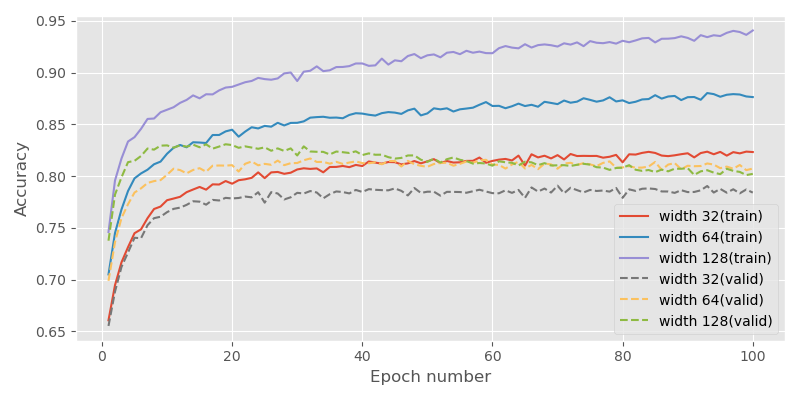
\includegraphics[width=\linewidth]{figures/acc_curves_width.png}
        \caption{accuracy by epoch}
        \label{fig:width_acccurves}
    \end{subfigure} 
    \begin{subfigure}{\linewidth}
        \centering
        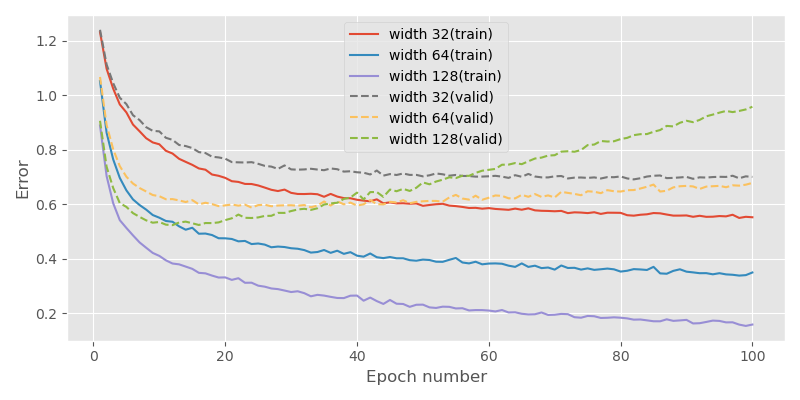
\includegraphics[width=\linewidth]{figures/error_curves_width.png}
        \caption{error by epoch}
        \label{fig:width_errorcurves}
    \end{subfigure} 
    \caption{Training and validation curves in terms of classification accuracy (a) and cross-entropy error (b) on the EMNIST dataset for different network widths.}
    \label{fig:width}
\end{figure} 
% }
}

%% Question Figure 3:
\newcommand{\questionFigureThree} {
% \youranswer{
%Question Figure 3 - Replace these images with figures depicting the accuracy and error, training and validation curves for your experiments varying the number of hidden layers.
%
\begin{figure}[t]
    \centering
    \begin{subfigure}{\linewidth}
        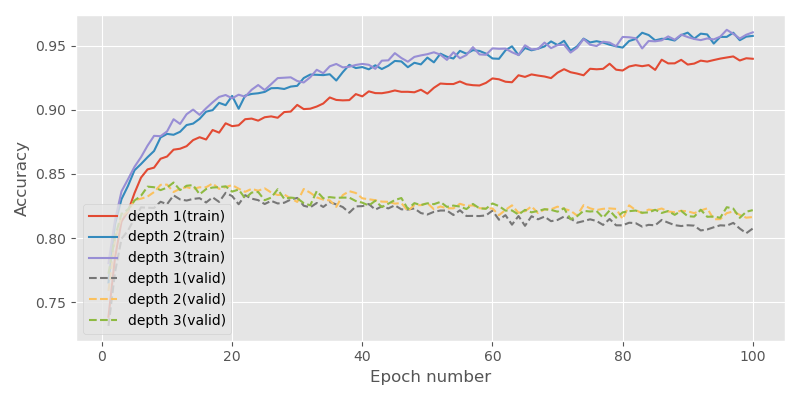
\includegraphics[width=\linewidth]{figures/acc_curves_height.png}
        \caption{accuracy by epoch}
        \label{fig:depth_acccurves}
    \end{subfigure} 
    \begin{subfigure}{\linewidth}
        \centering
        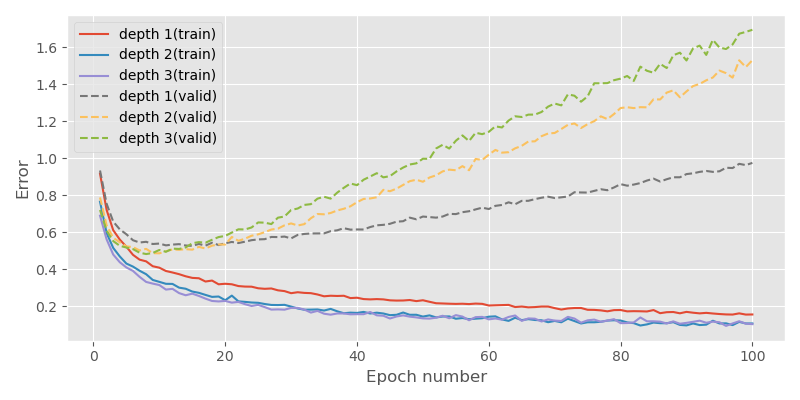
\includegraphics[width=\linewidth]{figures/error_curves_height.png}
        \caption{error by epoch}
        \label{fig:depth_errorcurves}
    \end{subfigure} 
    \caption{Training and validation curves in terms of classification accuracy (a) and cross-entropy error (b) on the EMNIST dataset for different network depths.}
    \label{fig:depth}
\end{figure} 
% }
}


%% Question Figure 4: Replace these images with figures depicting the Validation Accuracy and Generalisation Gap (difference between validation and training error) for each of the experiment results varying the Dropout inclusion rate, and L1/L2 weight penalty depicted in Table 3 (including any results you have filled in).
\newcommand{\questionFigureFour} {
% \youranswer{
%
\begin{figure*}[t]
    \centering
    \begin{subfigure}{.475\linewidth}
        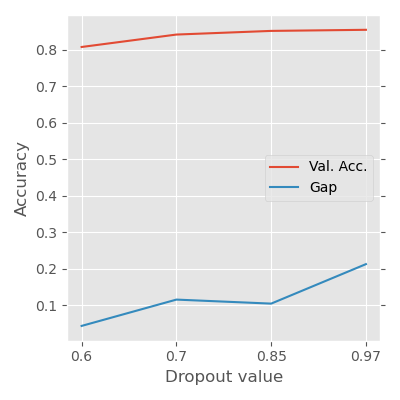
\includegraphics[width=\linewidth]{figures/dropout_plot.png}
        \caption{Accuracy and error gap with varying dropout values.}
        \label{fig:dropoutrates}
    \end{subfigure} 
    \begin{subfigure}{.475\linewidth}
        \centering
        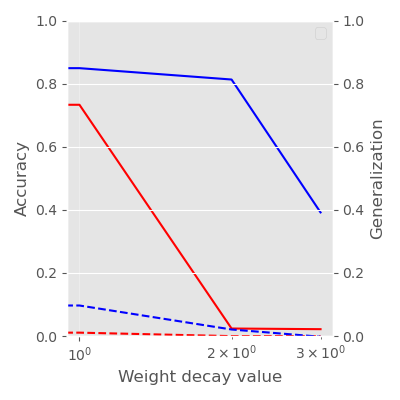
\includegraphics[width=\linewidth]{figures/wd_plot.png}
        \caption{Accuracy and error gap by weight penalty.}
        \label{fig:weightrates}
    \end{subfigure} 
    \caption{Accuracy and error by regularisation strength of each method (Dropout and L1/L2 Regularisation).}
    \label{fig:hp_search}
\end{figure*}
% }
}

%% Question Figure 5:Question Figure 5 - Add figures depicting the Validation Accuracy and Generalisation Gap (difference between validation and training error) for each of your 4 experiments  varying your hyperparameters for the combination of L1 and L2 regularisation (based on your implementation) depicted in Table 4.
\newcommand{\questionFigureFive} {
% \youranswer{
    \begin{figure*}[t]
    \centering
    \begin{subfigure}{.475\linewidth}
        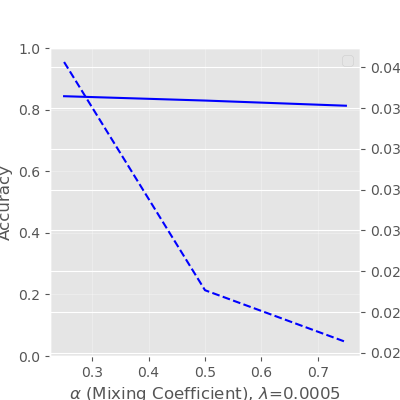
\includegraphics[width=\linewidth]{figures/mix_wd_alpha_plot.png}
        \caption{Accuracy and error gap for varying mixing ratio values.}
        \label{fig:wd-alpha}
    \end{subfigure} 
    \begin{subfigure}{.475\linewidth}
        \centering
        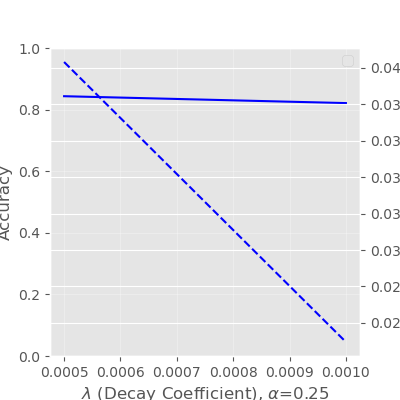
\includegraphics[width=\linewidth]{figures/mix_wd_lambda_plot.png}
        \caption{Accuracy and error by weight penalty.}
        \label{fig:wd-lambda}
    \end{subfigure} 
    \caption{Accuracy and error by regularisation strength and misxing penalty respectively of combined L1 and L2 Regularisation.}
    \label{fig:lamda_alpha_wd}
\end{figure*}
% }
}

%% Question Figure 6:Add figures depicting the Training Accuracy, Error, and Gradient Flow Across Layers for the 1 experiment run with the Custom Activation function (produce these by running the "Problematic Training" cell in the Coursework\_1.ipynb notebook).
\newcommand{\questionFigureSix} {
% \youranswer{
        \begin{figure*}[t]
    \centering
    \begin{subfigure}{.475\linewidth}
        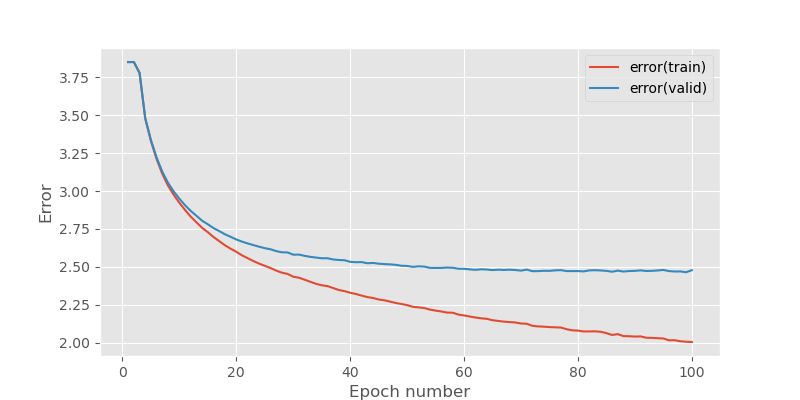
\includegraphics[width=\linewidth]{figures/custom_activation_error_plot.png}
        \caption{Training Error and Validation Error curves for the Custom Activation function experiment.}
        \label{fig:custom-activation-error}
    \end{subfigure}
    \begin{subfigure}{.475\linewidth}
        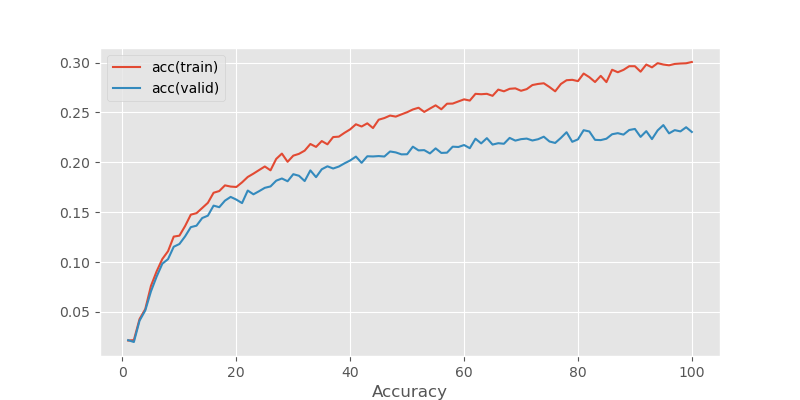
\includegraphics[width=\linewidth]{figures/custom_activation_accuracy_plot.png}
        \caption{Training Accuracy and Validation Accuracy curves for the Custom Activation function experiment.}
        \label{fig:custom-activation-accuracy}
    \end{subfigure} 
    \begin{subfigure}{.475\linewidth}
        \centering
        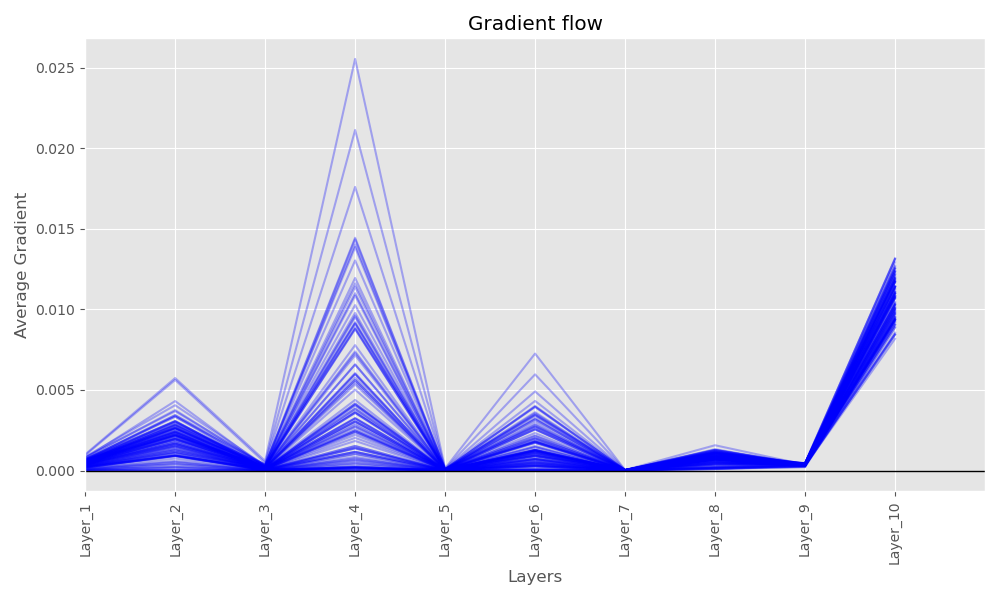
\includegraphics[width=\linewidth]{figures/custom_activation_grad_flow_plot.png}
        \caption{Gradient Flow Across Layers for the Custom Activation function experiment.}
        \label{fig:custom-activation-gradflow}
    \end{subfigure} 
    \caption{Figures depicting the Training Accuracy, Error, and Gradient Flow Across Layers for the 1 experiment run with the Custom Activation function}
    \label{fig:custom-activation}
\end{figure*}
% }
}

%% - - - - - - - - - - - - TABLES - - - - - - - - - - - - 

%% Question Table 1:
\newcommand{\questionTableOne} {
% \youranswer{
%Question Table 1 - Fill in Table 1 with the results from your experiments varying the number of hidden units.
%
\begin{table}[t]
    \centering
    \begin{tabular}{c|ccc}
    \toprule
        \# Hidden Units & Val. Acc. & Train Error & Val. Error\\
    \midrule
         32            &    79.0\%   &  0.552 &   0.700            \\
         64            &    80.7\%   &  0.350  &   0.678               \\
         128           &    80.2\%   &  0.156  &   0.973           \\ 
    \bottomrule
    \end{tabular}
    \caption{Validation accuracy (\%) and training/validation error (in terms of cross-entropy error) for varying network widths on the EMNIST dataset.}
    \label{tab:width_exp}
\end{table}
% }
}

%% Question Table 2:
\newcommand{\questionTableTwo} {
% \youranswer{%Question Table 2 - Fill in Table 2 with the results from your experiments varying the number of hidden layers.
%
\begin{table}[t]
    \centering
    \begin{tabular}{c|ccc}
    \toprule
        \# Hidden Layers & Val. Acc. & Train Error & Val. Error \\
    \midrule
         1 & 0.807 & 0.156 & 0.975 \\
         2 & 0.816 & 0.107 & 1.529 \\
         3 & 0.822 & 0.104 & 1.693 \\ 
    \bottomrule
    \end{tabular}
    \caption{Validation accuracy (\%) and training/validation error (in terms of cross-entropy error) for varying network depths on the EMNIST dataset.}
    \label{tab:depth_exps}
\end{table}
% }
}

%% Question Table 3:
\newcommand{\questionTableThree} {
% \youranswer{
% Question Table 3 - Fill in Table 3 with the results from your experiments for the missing hyperparameter values for each of L1 regularisation, L2 regularisation, Dropout and label smoothing (use the values shown on the table).
%
\begin{table*}[t]
    \centering
    \begin{tabular}{c|c|ccc}
    \toprule
        Model    &  Hyperparameter value(s) & Validation accuracy & Train Error & Validation Error \\
    \midrule
    \midrule
        Baseline &  -                    &               0.837 &       0.241 &  0.533          \\
    \midrule
        \multirow{4}*{Dropout}
                 & 0.6                   &  80.7                &      0.549 & 0.593     \\
                 & 0.7 & 0.841 & 0.348 & 0.464  \\
                 & \textbf{\textit{0.85}} & \textbf{\textit{85.1}} &  \textbf{\textit{0.329}} & \textbf{\textit{0.434}} \\
                 & 0.97 & 85.4 &  0.244 & 0.457  \\
    \midrule
        \multirow{4}*{L1 penalty}
                 & \textit{5e-4} & \textit{79.5} & \textit{0.642} & \textit{0.658} \\
                 & 1e-3 & 0.733 & 0.883 & 0.894 \\
                 & 5e-3 & 2.41 & 3.850 & 3.850 \\
                 & 5e-2 & 2.20 & 3.850 & 3.850 \\
    \midrule
        \multirow{4}*{L2 penalty}  
                 & 5e-4 & 85.1 & 0.306 & 0.460 \\
                 & \textit{1e-3} & \textit{0.849} & \textit{0.356} & \textit{0.453} \\
                 & 5e-3 & 81.3 & 0.586 & 0.607 \\
                 & 5e-2 & 39.2 & 2.258 & 2.256  \\
    \midrule
        Label smoothing & 0.1 & 0.853 & 1.020 & 0.557 \\
    \bottomrule
    \end{tabular}
    \caption{Results of all hyperparameter search experiments. \emph{italics} indicate the best results per series (Dropout, L1 Regularisation, L2 Regularisation, Label smoothing) and \textbf{bold} indicates the best overall.}
    \label{tab:hp_search}
\end{table*}
% }
}


%% Question Table 4: Add a table with the results from your 4 experiments (by which we mean: 4 training runs, NOT 4 sets of experiments) varying your hyperparameters for the combination of L1 and L2 regularisation (based on your implementation).
\newcommand{\questionTableFour} {
% \youranswer{
    \begin{table*}[t]
    \centering
    \begin{tabular}{c|cc|ccc}
    \toprule
        Model    & \multicolumn{2}{c|}{Hyperparameters} & Validation accuracy & Train Error & Validation Error \\
                  & $\lambda$ &$\alpha$ & & & \\
    \midrule
    \midrule
        Baseline &  --  &   -- & 0.837 &  0.241 &  0.533  \\
    \midrule
        \multirow{4}*{L1 and L2 penalty mixed}
                 & \textbf{$\bm{5\times 10^{-4}}$} & \textbf{0.25} &  \textbf{0.843} & \textbf{0.437} & \textbf{0.477}     \\
                 & $5\times 10^{-4}$ & 0.50 & 0.829 & 0.505 & 0.532  \\
                 & $5\times 10^{-4}$ & 0.75 & 0.813 &  0.587 &  0.610 \\
                 & $1\times 10^{-3}$ & 0.25 & 0.821 &  0.538 & 0.563  \\
    \bottomrule
    \end{tabular}
    \caption{Results of all hyperparameter search experiments for combined L1 and L2 regularisation. \textbf{bold} indicates the best results for this experiment. $\lambda$ is our hyperparameter controlling the overall strength of regularisation, while $\alpha$ is the mixing coefficient, which controls the balance between L1 and L2 penalties.}
    \label{tab:l1l2_hp_search}
\end{table*}
% }
}

\newcommand{\appendixMixupCutMix}{
\youranswer{\section*{Appendix: Mixup and CutMix on EMNIST}\label{apx:mixup-cutmix}
\textbf{Setup.} 3-layer MLP (ReLU, hidden width 128), Softmax output, Adam optimiser. Initial runs at learning rate $10^{-2}$ diverged; the follow-up sweep used learning rate $3\times10^{-4}$, batch size $256$, $100$ epochs. Data augmentation used Mixup and CutMix via \texttt{MixupCutmixDataProvider} (Beta-$\alpha$ sampling with permutation and CutMix area correction); loss was CrossEntropy with soft labels.

\textbf{Configurations.}
\begin{table}[h]
    \centering
    \small
    \begin{tabular}{l|ccc|c}
        \toprule
        Run & Train err. & Val. err. & Val. Acc. & Runtime (s) \\
        \midrule
        baseline\_lr3e-4   & 3.320 & 3.363 & 0.523 & 289 \\
        mixup\_a0.4        & 3.364 & 3.280 & 0.607 & 307 \\
        cutmix\_a0.8       & 3.484 & 3.309 & 0.577 & 305 \\
        mix+cut\_combo     & 3.425 & 3.302 & 0.585 & 310 \\
        \bottomrule
    \end{tabular}
    \caption{Mixup/CutMix ablations (learning rate $3\times10^{-4}$, batch size 256, 100 epochs).}
    \label{tab:mixup_cutmix_results}
\end{table}

\textbf{Outcome.} All runs remained near-chance performance (chance $\approx 2\%$ for 47 classes): training error $\sim 3.3$ (vs. $3.85$ for uniform softmax) and validation accuracy $\leq 0.61$. The augmentation code includes (Beta-$\alpha$ sampling, permutation, CutMix area-adjusted labels); the bottleneck is optimisation and capacity: the MLP barely learns before augmentation is applied.

\textbf{Fixes proposed for follow-up.} (i) Lower learning rate to $1\times10^{-4}$ (or $7\times10^{-5}$ if still unstable); (ii) increase width to $256$ and optionally insert \texttt{DropoutLayer} (incl\_prob $0.8$) after each ReLU for stable training; (iii) enable label smoothing on train only (\texttt{smooth\_labels=True}) to stabilise soft targets; (iv) reduce augmentation strength: Mixup $\alpha=0.8$, prob $0.7$; CutMix $\alpha=1.0$, prob $0.5$; Combo Mixup $\alpha=0.4$ + CutMix $\alpha=0.8$, probs $0.5/0.3$. Expectation: recover $\sim$0.8+ validation accuracy baseline and allow Mixup/CutMix to add modest gains once the optimiser is stable.}
}

%% END of YOUR ANSWERS
